% http://www.thecartech.com/subjects/machine_elements_design/keys_and_Splines.htm

\section{Shaft Fixtures and Fittings}

This section provides descriptions of a few fixtures and methods of fitting components to a shaft. You may need to use this in your exercise as well as performing your own research on other techniques that might be suitable.

\subsection{Spline}

\begin{marginfigure}
    \centering
    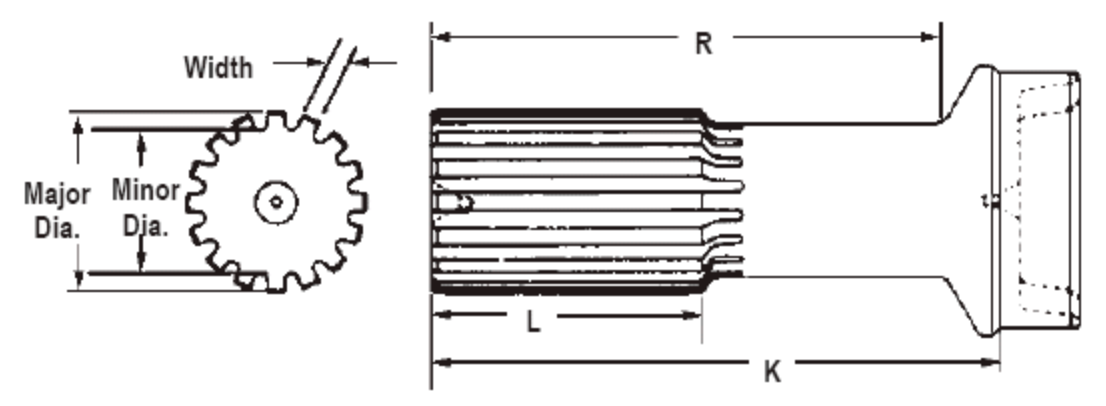
\includegraphics[width=\textwidth]{09_fixtures_and_fittings/spline-shaft.png}
    \caption{Spline shaft}
\end{marginfigure}
Splines are ridges or teeth on a drive shaft that mesh with grooves in a mating piece. This enables the transfer of high torque loads, whilst maintaining angular correspondence. There are a number of different types including:

\begin{itemize}
    \item Parallel key spline
    \item Involute spline
    \item Crowned splines
    \item Serrations
    \item Helical splines
    \item Ball splines
\end{itemize}

Here are some calculations often used for splines\sidenote{\url{http://www.thecartech.com/subjects/machine_elements_design/keys_and_Splines.htm}}.

The first is the calculation of the Torque capacity for a spline and this is given by:\marginnote{Torque Capacity of Spline}

\begin{equation}
    T=pAr_m
\end{equation}

\noindent where:

\begin{description}
    \item[\( p \)] Permissibale pressure on the splines (\(<7\si{\mega\pascal}\), if relative axial motion)
    \item[\(A\)] Total load area of splines (\(0.5(D-d)Ln\), \si{\metre^2})
    \item[\(D\)] Outer spline shaft diameter (\si{\metre})
    \item[\(d\)] Inner spline shaft diameter (\si{\metre})
    \item[\(L\)] Length of spline (\si{\metre})
    \item[\(n\)] Number of splines
    \item[\(r_m\)] Mean radius (\si{\metre})
\end{description}

The shear that a spline experiences can be calculated as follows:\marginnote{Spline Shear}

\begin{equation}
    \tau = \frac{4T}{Lbn(D+d)}
\end{equation}

where:

\begin{description}
    \item[\( F \)] Force acting on a spline 
    \item[\( b \)] Spline width
    \item[\( n \)] Number of splines
\end{description}


%\marginnote{Spline in Bending}

%\begin{equation}
%  \sigma_b = \frac{3F(D-d)}{b^2Ln}
%\end{equation}

%\marginnote{Pressure on groove supporting surface} 

%\begin{equation}
%  d_{\min} = \sqrt[3]{\frac{16T K_a S_v}{\pi{} \tau K_f}}
%\end{equation}

%where:

%\begin{description}
%  \item[\( d_{\min} \)] Minimal shaft diameter
%  \item[\(T\)] Torque (\si{\newton\metre})
%  \item[\(K_a\)] Application factor
%  \item[\(K_f\)] Fatigue-life factor
%  \item[\(S_v\)] Desired safety
%  \item[\(\tau\)] Allowable shear stress (\si{\pascal})
%\end{description}


\subsection{Taper Lock} 

\begin{marginfigure}
    \centering
    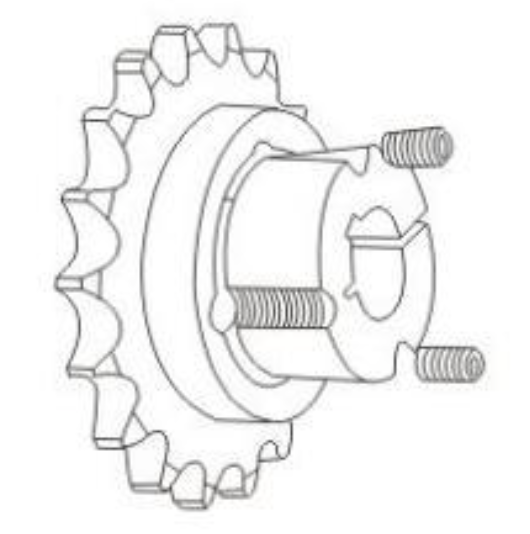
\includegraphics[width=\textwidth]{09_fixtures_and_fittings/taper-lock.png}
    \caption{Taper lock}
\end{marginfigure}
The Taper Lock bush, also referred to as a Taper bush or Taper Fit bush, is a locking mechanism commonly used in Power Transmission Drives for locating pulleys, sprockets, and couplings to shafts. 
The Taper Lock bush is pre-bored and keyed to match the required shaft and keyway diameters. 
The outside of the bush is tapered to match the component bore that is to be located on the shaft.

\subsection{Keyway} 

Keyways are a common method of transmitting the torque from the shaft to an attached component such as a sprocket.

\begin{figure}[h!]
    \centering
    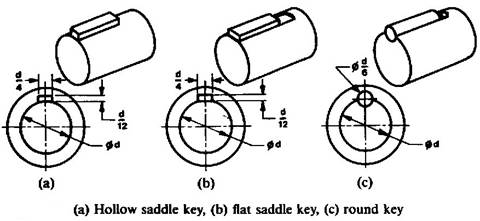
\includegraphics[width=\textwidth]{09_fixtures_and_fittings/keys.jpg}
    \caption{Types of key}
\end{figure}

When\marginnote{Determining the Minimum Key Size} a torque is applied, a key experiences two stress, a shear stress \(\tau\) and compressive stress \(\sigma_c\). These can be calculated as follows:

\marginnote{key shear (\(\tau\))}

\begin{equation}
  \tau = \frac{T}{wLr}
\end{equation}

\noindent{}Where:

\begin{description}
    \item[\(\tau\)] Key shear (\si{\pascal})
    \item[\(T\)] Torque (\si{\newton\metre})
    \item[\(w\)] Key width (\si{\metre})
    \item[\(L\)] Key length (\si{\metre})
    \item[\(r\)] Shaft radius (\si{\metre})
\end{description}

\marginnote{Key Compressive Stress (\(\sigma_c\))}

\begin{equation}
    \sigma_c = \frac{T}{0.5tLr}
\end{equation}

\noindent{}Where:

\begin{description}
    \item[\(\sigma_c\)] Compressive stress (\si{\pascal})
    \item[\(T\)] Torque (\si{\newton\metre})
    \item[\(t\)] Key height (\si{\metre})
    \item[\(L\)] Key length (\si{\metre})
    \item[\(r\)] Shaft radius (\si{\metre})
\end{description}

\marginnote{Standard Key Sizes} Although you can calculate the exact dimensions required for your key, there are standards for key sizes. Therefore, you can select any that meet your minimum requirements.

\begin{figure}[h!]
    \centering
    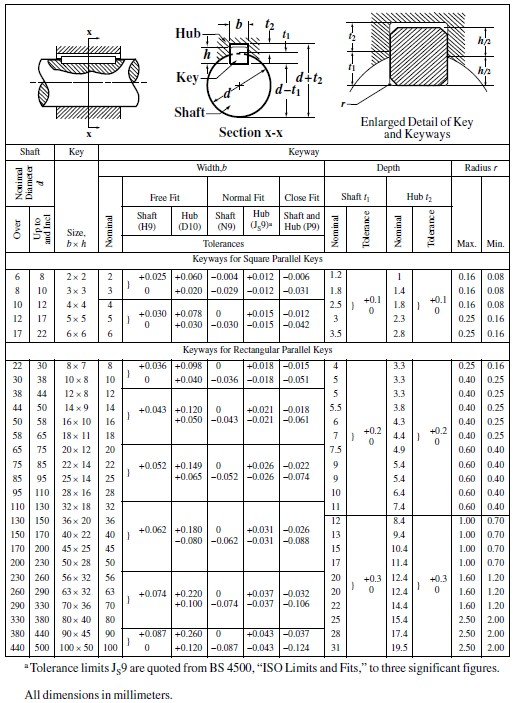
\includegraphics[width=0.8\textwidth]{09_fixtures_and_fittings/key-selection.jpg}
    \caption{An example of a key selection chart}
\end{figure}

\subsection{Circlip}

Circlips are a type of fastener consisting of a semi-flexible metal ring with open ends, which can be snapped into a machined groove on a dowel pin or other part to permit rotation but to prevent lateral movement. 
There are two basic types: internal and external, referring to whether they are fitted into a bore or over a shaft.
Circlips are often used to secure pinned connections.
There are many vendors that can provide circlips and provide information such as the one in \cref{tbl-circlip} to aid in the selection of the appropriate size clip for your needs.

\begin{table}[h!]
    \caption{An example of an external circlip information sheet}\label{tbl-circlip}
    \centering
    \scriptsize
    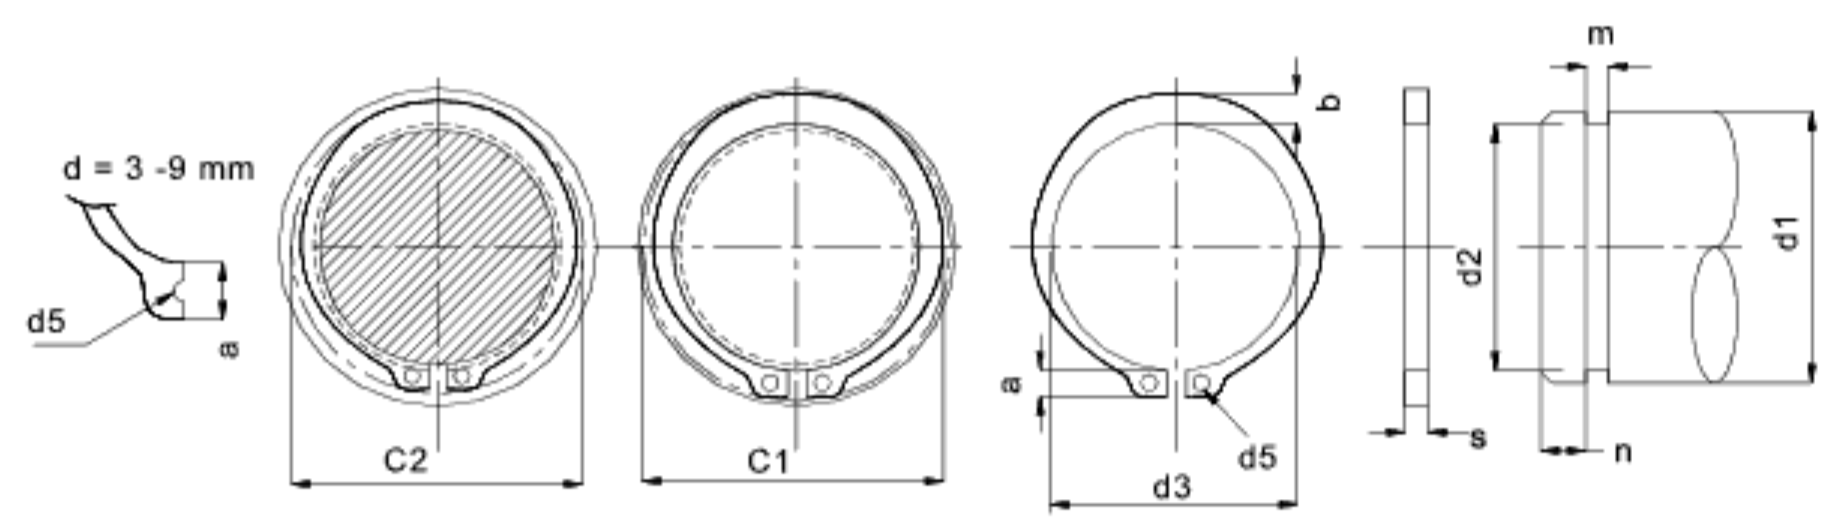
\includegraphics[width=0.8\textwidth]{09_fixtures_and_fittings/circlip-dimensions.png}
    \begin{tabular}{r r r r r r r r r r r r r r r r r}
    \toprule
    \multicolumn{1}{p{0.05\textwidth}}{Nom size (\si{\milli\metre})} & 
    \multicolumn{9}{c}{Circlip Dimensions (\si{\milli\metre})} &
    \multicolumn{5}{c}{Groove Dimensions (\si{\milli\metre})} & 
    \multicolumn{1}{p{0.05\textwidth}}{Groove Strength} & 
    \multicolumn{1}{p{0.05\textwidth}}{Circlip Strength} \\
    \midrule
    $d_1$ & $s$ & $s$ (tol) & $d_3$ & $d_3$ (tol) & $a_{\max}$ & $b$ & $d_{\min}$ & $C1$ & $C2$ & $d_2$ & $d_2$ (tol) & $m_{min}$ & $t$ & $n$ & $F_n$ (kN) & $F_r$ (kN) \\
    \midrule
    
    17 & 1,00 & 0,00 & 15,7 & +0,10 & 3,8 & 2,3 & 1,7 & 25,0 & 23,8 & 16,2 & 0,00 & 1,10 & 0,40 & 1,2 & 3,4 & 8,0 \\
    & & -0,06 & & -0,43 & & & & & & & -0,11 & & & & & \\
    
    18 & 1,20 & 0,00 & 16,5 & +0,10 & 3,9 & 2,4 & 2,0 & 26,2 & 24,8 & 17,0 & 0,00 & 1,30 & 0,50 & 1,5 & 4,5 & 17,00 \\
    & & -0,06 & & -0,44 & & & & & & & -0,11 & & & & & \\
    
    19 & 1,20 & 0,00 & 17,5 & +0,10 & 3,9 & 2,5 & 2,0 & 27,2 & 25,8 & 18,0 & 0,00 & 1,30 & 0,50 & 1,5 & 4,5 & 17,00 \\
    & & -0,06 & & -0,45 & & & & & & & -0,11 & & & & & \\
    
    \multicolumn{17}{c}{\ldots} \\
    
    \bottomrule
    
    \end{tabular}
\end{table}

